\documentclass[../../main.tex]{subfiles}

\graphicspath{{../../image/}{../../figure/}}

\begin{document}

\section{决策理论}\label{section:ch04-决策理论}

我们将回归任务看作条件概率分布$p(t\mid\boldsymbol{x})$来建模，并且选择了条件概率的特定形式，即Gauss分布[式\eqref{align:ch04-条件Gauss}]，其中与$\boldsymbol{x}$相关的均值$y(\boldsymbol{x},\boldsymbol{w})$由参数$\boldsymbol{w}$控制，方差由参数$\sigma^2$给出。$\boldsymbol{w}$和$\sigma^2$都可以使用最大似然从数据中学习得到。预测分布（predictive distribution）的结果如下：

\begin{align}
  p(t\mid\boldsymbol{x},\boldsymbol{w}_{\mathrm{ML}},\sigma^2_{\mathrm{ML}})=\mathcal{N}\bigl(t\mid y(\boldsymbol{x},\boldsymbol{w}_{\mathrm{ML}}),\sigma^2_{\mathrm{ML}}\bigr)
  \label{align:ch04-预测分布}
\end{align}

预测分布表达了我们对某些新输入$\boldsymbol{x}$所对应$t$值的不确定性。然而，对于许多实际应用，我们需要预测$t$的具体值，而不是返回整个分布，特别是在需要采取特定行动的情况下。例如，如果我们想要确定用于治疗肿瘤的最佳辐射水平，而我们的模型预测了辐射剂量的概率分布，那么我们必须使用该分布来决定给予治疗的具体剂量。因此，我们的任务分为两个阶段。第一个阶段称为推理（inference）阶段，我们使用训练数据来确定预测分布$p(t\mid\boldsymbol{x})$。第二个阶段称为决策（decision）阶段，我们使用这个预测分布来确定特定的值$f(\boldsymbol{x})$。这个特定的值依赖于输入向量$\boldsymbol{x}$，并且根据某些准则是最优的。我们可以通过最小化一个既依赖于预测分布$p(t\mid\boldsymbol{x})$又依赖于特定值$f(\boldsymbol{x})$的损失函数（也称成本函数）来实现这一点。

直觉上，我们可以选择条件分布的均值，即$f(\boldsymbol{x})=y(\boldsymbol{x},\boldsymbol{w}_{\mathrm{ML}})$。在某些情况下，这种直觉是正确的；但在其他情况下，它可能会给出非常糟糕的结果。因此，我们需要将其形式化，这样我们就可以理解它应该何时应用以及在什么假设下应用。该框架称为决策理论（decision theory）。

假设真实值为$t$，我们为预测选择了一个值$f(\boldsymbol{x})$，从而得到某种形式的惩罚或成本。惩罚是由损失（loss）决定的，用$L(t,f(\boldsymbol{x}))$表示。当然，由于我们不知道$t$的真实值，因此我们并不最小化$L$本身，而是最小化平均或期望的损失。

\begin{definition}[损失函数与期望损失]\label{definition:ch04-损失函数}
设$L(t,f(\boldsymbol{x}))$为预测值$f(\boldsymbol{x})$与真实值$t$之差的\textbf{损失函数}（也称成本函数）。由于$t$未知，我们最小化的不是$L$本身，而是以联合分布$p(\boldsymbol{x},t)$为权重的平均或期望损失
\begin{align}
  \mathbb{E}[L]=\iint L(t,f(\boldsymbol{x}))\,p(\boldsymbol{x},t)\,\mathrm{d}\boldsymbol{x}\,\mathrm{d}t,
  \label{align:ch04-期望损失}
\end{align}
其中，我们以输入变量和目标变量的联合分布$p(\boldsymbol{x},t)$作为权重对它们的分布进行加权平均。
\end{definition}

% SUPPLEMENT: parent=definition:ch04-损失函数; kind=motivation; location=紧随其后的 remark（重构新增）
\begin{remark}（重构新增）
\cref{definition:ch04-损失函数}把“预测得好不好”这件事拆成了两个独立的成分：损失函数$L$刻画\emph{错多少算多严重}，联合分布$p(\boldsymbol{x},t)$刻画\emph{什么样的$({\boldsymbol{x}},t)$更常出现}。\eqref{align:ch04-期望损失}把二者以加权平均的方式合成一个标量，从而使“选择$f$”变成一个可以优化的目标。

这一形式化的代价是：最小化$\mathbb{E}[L]$要求知道$p(\boldsymbol{x},t)$，而实际只掌握训练数据和\cref{section:ch04-决策理论}开头给出的预测分布。因此\eqref{align:ch04-期望损失}在理论上定义了“最优”，在下文中只作为推导最优决策规则的出发点，并不直接作为可计算的训练目标。

注意$\mathbb{E}[L]$中的期望是对$({\boldsymbol{x}},t)$的联合分布取的，因而同时包含了$t$的随机性和$\boldsymbol{x}$的分布。若$p(\boldsymbol{x})$在某个区域为零，则该区域上的$f$取值不影响$\mathbb{E}[L]$——这一点在讨论最优解的\emph{唯一性}时必须注意。
\end{remark}

回归问题中常见的损失函数是平方损失函数：$L(t,f(\boldsymbol{x}))=\{f(\boldsymbol{x})-t\}^2$。在这种情况下，期望损失函数可以写成

\begin{align}
  \mathbb{E}[L]=\iint\{f(\boldsymbol{x})-t\}^2p(\boldsymbol{x},t)\,\mathrm{d}\boldsymbol{x}\,\mathrm{d}t
  \label{align:ch04-平方损失期望}
\end{align}

注意不要将平方损失函数与前面介绍的平方和误差函数弄混淆。误差函数用于在训练过程中设置参数，以便确定条件概率分布$p(t\mid\boldsymbol{x})$，而损失函数则控制如何使用条件分布来达到预测函数$f(\boldsymbol{x})$，以预测$\boldsymbol{x}$的每个值。

我们的目标是找到能使$\mathbb{E}[L]$最小的$f(\boldsymbol{x})$。假设$f(\boldsymbol{x})$是一个完全任意的函数，则可以使用变分法（参见\cref{definition:appB-泛函导数}）得到

\begin{align}
  \frac{\delta\mathbb{E}[L]}{\delta f(\boldsymbol{x})}=2\int\{f(\boldsymbol{x})-t\}p(\boldsymbol{x},t)\,\mathrm{d}t=0
  \label{align:ch04-损失变分}
\end{align}

\begin{proposition}[平方损失的最优决策规则]\label{proposition:ch04-最优决策规则}
设$\mathbb{E}[L]$由\eqref{align:ch04-平方损失期望}给出，$f$在所有满足所需可积性的函数中选取。则$\mathbb{E}[L]$的驻点满足\eqref{align:ch04-损失变分}，且最优解为条件平均
\begin{align}
  f^*(\boldsymbol{x})=\frac{1}{p(\boldsymbol{x})}\int t\,p(\boldsymbol{x},t)\,\mathrm{d}t=\int t\,p(t\mid\boldsymbol{x})\,\mathrm{d}t=\mathbb{E}_t[t\mid\boldsymbol{x}],
  \label{align:ch04-回归函数}
\end{align}
即可取$f^*(\boldsymbol{x})=\mathbb{E}_t[t\mid\boldsymbol{x}]$。
\end{proposition}

\begin{proof}
（重构新增）第一步，写出变分条件。令$f$作扰动$f+\varepsilon\eta$，由\eqref{align:ch04-平方损失期望}，
\begin{align*}
  \mathbb{E}[L]&=\iint\bigl\{f(\boldsymbol{x})+\varepsilon\eta(\boldsymbol{x})-t\bigr\}^2p(\boldsymbol{x},t)\,\mathrm{d}\boldsymbol{x}\,\mathrm{d}t\\
  &=\mathbb{E}[L]\big|_{f}+\varepsilon\iint2\{f(\boldsymbol{x})-t\}\eta(\boldsymbol{x})p(\boldsymbol{x},t)\,\mathrm{d}\boldsymbol{x}\,\mathrm{d}t+O(\varepsilon^2),
\end{align*}
与泛函导数的定义（见\cref{definition:appB-泛函导数}）比较，得
\begin{align*}
  \frac{\delta\mathbb{E}[L]}{\delta f(\boldsymbol{x})}=2\int\{f(\boldsymbol{x})-t\}p(\boldsymbol{x},t)\,\mathrm{d}t,
\end{align*}
令其为零即得\eqref{align:ch04-损失变分}。

第二步，解出$f(\boldsymbol{x})$。在\eqref{align:ch04-损失变分}中把含$f(\boldsymbol{x})$的项与不含的项分开（$f(\boldsymbol{x})$对$t$的积分是常数）：
\begin{align*}
  f(\boldsymbol{x})\int p(\boldsymbol{x},t)\,\mathrm{d}t=\int t\,p(\boldsymbol{x},t)\,\mathrm{d}t.
\end{align*}
由概率的加和法则，$\int p(\boldsymbol{x},t)\,\mathrm{d}t=p(\boldsymbol{x})$，故当$p(\boldsymbol{x})>0$时
\begin{align*}
  f(\boldsymbol{x})=\frac{1}{p(\boldsymbol{x})}\int t\,p(\boldsymbol{x},t)\,\mathrm{d}t.
\end{align*}

第三步，化为条件平均。由乘积法则$p(\boldsymbol{x},t)=p(t\mid\boldsymbol{x})p(\boldsymbol{x})$，
\begin{align*}
  \frac{1}{p(\boldsymbol{x})}\int t\,p(\boldsymbol{x},t)\,\mathrm{d}t
  =\frac{1}{p(\boldsymbol{x})}\int t\,p(t\mid\boldsymbol{x})p(\boldsymbol{x})\,\mathrm{d}t
  =\int t\,p(t\mid\boldsymbol{x})\,\mathrm{d}t=\mathbb{E}_t[t\mid\boldsymbol{x}],
\end{align*}
此即\eqref{align:ch04-回归函数}。

第四步，说明这是最小值而非最大值。由\eqref{align:ch04-平方损失分解}（其证明见\cref{proposition:ch04-期望损失分解}），$\mathbb{E}[L]$等于一个只依赖于$f$的非负项加上一个与$f$无关的常数项，而该非负项在$f=f^*$处取零，故$f^*$给出全局最小值。
\end{proof}

% SUPPLEMENT: parent=proposition:ch04-最优决策规则; kind=motivation; location=紧随其后的 remark（重构新增）
\begin{remark}（重构新增）
\cref{proposition:ch04-最优决策规则}的结论\eqref{align:ch04-回归函数}是本章从“概率”走向“决策”的关键一步：一旦损失取平方，最优预测就与$p(t\mid\boldsymbol{x})$的全部信息无关，只依赖它的\emph{一阶矩}。

这解释了为什么在\cref{definition:ch04-加性Gauss噪声}这样的模型下，\cref{subsection:ch04-最大似然}给出的$y(\boldsymbol{x},\boldsymbol{w}_{\mathrm{ML}})$恰好就是最优决策——因为Gauss分布的均值就是它的唯一参数。但它同时暴露了平方损失的局限：若$p(t\mid\boldsymbol{x})$是多峰的，条件均值可能落在两个峰之间的低密度区，此时$f^*$虽然在期望意义下最优，却几乎不可能是一个“典型”的$t$值。

推导中$\mathbb{E}[L]$对$f$的驻点条件是逐点成立的：\eqref{align:ch04-损失变分}对每个$\boldsymbol{x}$分别给出一个方程，这正是变分法“逐点变分”的含义。因此\eqref{align:ch04-回归函数}只在$p(\boldsymbol{x})>0$处被确定；在$p(\boldsymbol{x})=0$处$f$可以任意取值而不影响$\mathbb{E}[L]$。
\end{remark}

\begin{definition}[回归函数]\label{definition:ch04-回归函数}
\eqref{align:ch04-回归函数}给出的条件平均$\mathbb{E}_t[t\mid\boldsymbol{x}]$称为\textbf{回归函数}（regression function）。
\end{definition}

% SUPPLEMENT: parent=definition:ch04-回归函数; kind=motivation; location=紧随其后的 remark（重构新增）
\begin{remark}（重构新增）
回归函数$\mathbb{E}_t[t\mid\boldsymbol{x}]$只依赖条件分布$p(t\mid\boldsymbol{x})$，不依赖任何特定的损失函数，因此可以作为“给定$\boldsymbol{x}$时$t$的典型值”的通用刻画。\cref{proposition:ch04-最优决策规则}说明，在平方损失下它同时是最优预测；而在其他损失下最优预测可能是别的泛函（$q=1$时为条件中位数，$q\to0$时为条件众数，见\cref{definition:ch04-Minkowski损失}与\cref{exercise:ch04-12}）。

区分“回归函数”与“模型$y(\boldsymbol{x},\boldsymbol{w})$”是本章的一个基本区分：前者由数据生成机制$p(t\mid\boldsymbol{x})$决定，是拟合的对象；后者是拟合的工具，其参数$\boldsymbol{w}$由有限数据估计得到。二者的差距正是\cref{section:ch04-偏差方差权衡}要量化的偏差。
\end{remark}

结果如\cref{figure:ch04-回归函数}所示，这一形式可以很容易地扩展到由向量$\boldsymbol{t}$表示的多个目标变量。这时，最优解是条件平均$f^*(\boldsymbol{x})=\mathbb{E}_t[\boldsymbol{t}\mid\boldsymbol{x}]$（见\cref{exercise:ch04-08}）。对于形如\eqref{align:ch04-条件Gauss}的Gauss条件分布，条件均值可以简化为

\begin{align}
  \mathbb{E}[t\mid\boldsymbol{x}]=\int t\,p(t\mid\boldsymbol{x})\,\mathrm{d}t=y(\boldsymbol{x},\boldsymbol{w})
  \label{align:ch04-Gauss条件均值}
\end{align}

\begin{figure}[htbp]
  \centering
  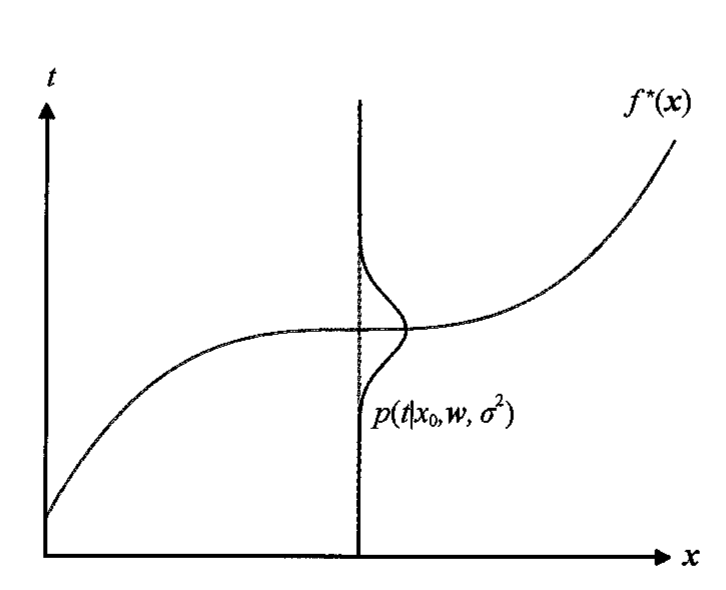
\includegraphics[width=0.5\textwidth]{ch04-fig4-5-regression-function.png}
  \caption{用于最小化期望平方损失的回归函数$f^*(\boldsymbol{x})$是由条件分布$p(t\mid\boldsymbol{x})$的均值给出的}
  \label{figure:ch04-回归函数}
\end{figure}

我们也可以用另一种推导方式得到这个结果，这种推导方式将阐明回归问题的本质。在知道最优解是条件期望的情况下，我们可以将平方项展开为

\begin{align}
  \{f(\boldsymbol{x})-t\}^2
  &=\bigl\{f(\boldsymbol{x})-\mathbb{E}[t\mid\boldsymbol{x}]+\mathbb{E}[t\mid\boldsymbol{x}]-t\bigr\}^2\nonumber\\
  &=\{f(\boldsymbol{x})-\mathbb{E}[t\mid\boldsymbol{x}]\}^2
  +2\{f(\boldsymbol{x})-\mathbb{E}[t\mid\boldsymbol{x}]\}\{\mathbb{E}[t\mid\boldsymbol{x}]-t\}
  +\{\mathbb{E}[t\mid\boldsymbol{x}]-t\}^2
  \label{align:ch04-平方项展开}
\end{align}

其中，为了保持符号整洁，我们使用$\mathbb{E}[t\mid\boldsymbol{x}]$来表示$\mathbb{E}_t[t\mid\boldsymbol{x}]$。代入损失函数\eqref{align:ch04-平方损失期望}并对$t$进行积分后，交叉项消失了，得到如下形式的损失函数的表达式：

\begin{proposition}[平方损失的期望损失分解]\label{proposition:ch04-期望损失分解}
设$\mathbb{E}[L]$由\eqref{align:ch04-平方损失期望}给出，且$p(\boldsymbol{x},t)$使所涉及的积分绝对收敛。则
\begin{align}
  \mathbb{E}[L]=\int\bigl\{f(\boldsymbol{x})-\mathbb{E}[t\mid\boldsymbol{x}]\bigr\}^2p(\boldsymbol{x})\,\mathrm{d}\boldsymbol{x}+\int\mathrm{var}[t\mid\boldsymbol{x}]\,p(\boldsymbol{x})\,\mathrm{d}\boldsymbol{x}
  \label{align:ch04-平方损失分解}
\end{align}
其中$\mathrm{var}[t\mid\boldsymbol{x}]\triangleq\mathbb{E}\bigl[\{t-\mathbb{E}[t\mid\boldsymbol{x}]\}^2\mid\boldsymbol{x}\bigr]$为给定$\boldsymbol{x}$时$t$的条件方差。
\end{proposition}

\begin{proof}
（重构新增）第一步，把\eqref{align:ch04-平方项展开}代回\eqref{align:ch04-平方损失期望}。三项分别记为$A$、$B$、$C$：
\begin{align*}
  \mathbb{E}[L]=\iint\{f(\boldsymbol{x})-\mathbb{E}[t\mid\boldsymbol{x}]\}^2p(\boldsymbol{x},t)\,\mathrm{d}\boldsymbol{x}\,\mathrm{d}t
  +\iint B\,p(\boldsymbol{x},t)\,\mathrm{d}\boldsymbol{x}\,\mathrm{d}t
  +\iint\{\mathbb{E}[t\mid\boldsymbol{x}]-t\}^2p(\boldsymbol{x},t)\,\mathrm{d}\boldsymbol{x}\,\mathrm{d}t.
\end{align*}

第二步，第一项对$t$积分。被积函数不含$t$，且$\int p(\boldsymbol{x},t)\,\mathrm{d}t=p(\boldsymbol{x})$，故
\begin{align*}
  \iint\{f(\boldsymbol{x})-\mathbb{E}[t\mid\boldsymbol{x}]\}^2p(\boldsymbol{x},t)\,\mathrm{d}\boldsymbol{x}\,\mathrm{d}t
  =\int\{f(\boldsymbol{x})-\mathbb{E}[t\mid\boldsymbol{x}]\}^2p(\boldsymbol{x})\,\mathrm{d}\boldsymbol{x}.
\end{align*}

第三步，交叉项$B$为零。先把$B$对$t$积分，注意$2\{f(\boldsymbol{x})-\mathbb{E}[t\mid\boldsymbol{x}]\}$不含$t$：
\begin{align*}
  \int B\,p(\boldsymbol{x},t)\,\mathrm{d}t
  &=2\{f(\boldsymbol{x})-\mathbb{E}[t\mid\boldsymbol{x}]\}\int\{\mathbb{E}[t\mid\boldsymbol{x}]-t\}p(\boldsymbol{x},t)\,\mathrm{d}t\\
  &=2\{f(\boldsymbol{x})-\mathbb{E}[t\mid\boldsymbol{x}]\}p(\boldsymbol{x})\int\{\mathbb{E}[t\mid\boldsymbol{x}]-t\}p(t\mid\boldsymbol{x})\,\mathrm{d}t\\
  &=2\{f(\boldsymbol{x})-\mathbb{E}[t\mid\boldsymbol{x}]\}p(\boldsymbol{x})\bigl\{\mathbb{E}[t\mid\boldsymbol{x}]-\mathbb{E}[t\mid\boldsymbol{x}]\bigr\}=0,
\end{align*}
其中第三步用了$\int p(t\mid\boldsymbol{x})\,\mathrm{d}t=1$与$\int t\,p(t\mid\boldsymbol{x})\,\mathrm{d}t=\mathbb{E}[t\mid\boldsymbol{x}]$。再对$\boldsymbol{x}$积分，$B$的贡献为零。

第四步，第三项$C$。由于$\{\mathbb{E}[t\mid\boldsymbol{x}]-t\}^2=\{t-\mathbb{E}[t\mid\boldsymbol{x}]\}^2$，且
\begin{align*}
  \iint\{t-\mathbb{E}[t\mid\boldsymbol{x}]\}^2p(\boldsymbol{x},t)\,\mathrm{d}\boldsymbol{x}\,\mathrm{d}t
  =\int\left(\int\{t-\mathbb{E}[t\mid\boldsymbol{x}]\}^2p(t\mid\boldsymbol{x})\,\mathrm{d}t\right)p(\boldsymbol{x})\,\mathrm{d}\boldsymbol{x},
\end{align*}
而内层积分按定义就是$\mathrm{var}[t\mid\boldsymbol{x}]$。

把第二步、第三步、第四步的结果代回第一步即得\eqref{align:ch04-平方损失分解}。
\end{proof}

% SUPPLEMENT: parent=proposition:ch04-期望损失分解; kind=motivation; location=紧随其后的 remark（重构新增）
\begin{remark}（重构新增）
\cref{proposition:ch04-期望损失分解}把\eqref{align:ch04-平方损失分解}的右端分成“可约”与“不可约”两部分，这一点对理解本章其余部分至关重要。

第一项只依赖于$f$，且非负，因此最小值为$0$，在$f(\boldsymbol{x})=\mathbb{E}[t\mid\boldsymbol{x}]$处取到——这正是\cref{proposition:ch04-最优决策规则}的另一种证法。第二项$\int\mathrm{var}[t\mid\boldsymbol{x}]p(\boldsymbol{x})\,\mathrm{d}\boldsymbol{x}$完全不含$f$，故任何预测函数都无法把它变小，它代表数据本身的内在噪声，是损失函数不可约的最小值。

推导中“交叉项为零”一步是全部技巧所在，而它成立的原因只有一条：$\mathbb{E}[t\mid\boldsymbol{x}]$是$t$在给定$\boldsymbol{x}$下的期望，故$t-\mathbb{E}[t\mid\boldsymbol{x}]$的条件期望为零。若把$\mathbb{E}[t\mid\boldsymbol{x}]$换成任何别的函数（例如条件中位数），交叉项一般不为零，分解式随之失效。

最后，本命题的绝对收敛假设不可省：若$\mathbb{E}[t^2]=\infty$，则$\mathbb{E}[L]$可能取$+\infty$，此时\eqref{align:ch04-平方损失分解}两端同时为$+\infty$，讨论最小值就失去了意义。
\end{remark}

我们需要确定的函数$f(\boldsymbol{x})$只出现在\eqref{align:ch04-平方损失分解}右侧的第一项中，当$f(\boldsymbol{x})$等于$\mathbb{E}[t\mid\boldsymbol{x}]$时，该项达到最小值。此时，\eqref{align:ch04-平方损失分解}右侧的这一项就消失了。这只是我们之前推导出来的结果，这表明最优最小二乘的预测是由条件均值给出的。\eqref{align:ch04-平方损失分解}右侧的第二项是分布$t$的方差在$\boldsymbol{x}$上取平均后的结果，代表目标数据的内在变化，可以视为噪声。因为它独立于$f(\boldsymbol{x})$，所以它代表损失函数不可约的最小值。

平方损失函数并不是回归中唯一可选的损失函数。平方损失的一种泛化形式称为Minkowski损失，其期望由下式给出：

\begin{definition}[Minkowski损失]\label{definition:ch04-Minkowski损失}
设$q>0$。称
\begin{align}
  \mathbb{E}[L_q]=\iint|f(\boldsymbol{x})-t|^q\,p(\boldsymbol{x},t)\,\mathrm{d}\boldsymbol{x}\,\mathrm{d}t
  \label{align:ch04-Minkowski损失}
\end{align}
为\textbf{Minkowski损失}的期望，它是平方损失的一种泛化形式。
\end{definition}

% SUPPLEMENT: parent=definition:ch04-Minkowski损失; kind=motivation; location=紧随其后的 remark（重构新增）
\begin{remark}（重构新增）
\cref{definition:ch04-Minkowski损失}以一个参数$q$统一了一族损失：$q=2$时\eqref{align:ch04-Minkowski损失}退化为\eqref{align:ch04-平方损失期望}，$q=1$时给出绝对误差，$q>2$时对大误差的惩罚更重，$q<1$时对大误差的惩罚反而变轻。

$q$的作用可以从\cref{figure:ch04-损失曲线}直接读出：$q$越小，曲线在$f=t$处的尖点越尖锐、在两侧越平坦，因此$q\to0$的极限只关心“$t$是否恰等于$f$”，这正是众数出现的机制；$q$越大，曲线越平坦而两侧越陡，因此对离群点越敏感。

需要说明的是，$q<1$时$|f-t|^q$不再是凸函数，\eqref{align:ch04-Minkowski损失}的最小化问题可能没有唯一解；本节的结论默认$q\geqslant1$，而\cref{exercise:ch04-12}讨论的$q\to0$极限应理解为$q\downarrow0$的极限行为。
\end{remark}

当$q=2$时即为期望平方损失。\cref{figure:ch04-损失曲线}给出了当$q$取不同值时，函数$|f-t|^q$关于$f-t$的曲线。$\mathbb{E}[L_q]$的最小值由$q=2$时的条件均值、$q=1$时的条件中位数和$q\to0$时的条件众数给出（见\cref{exercise:ch04-12}）。

\begin{figure}[htbp]
  \centering
  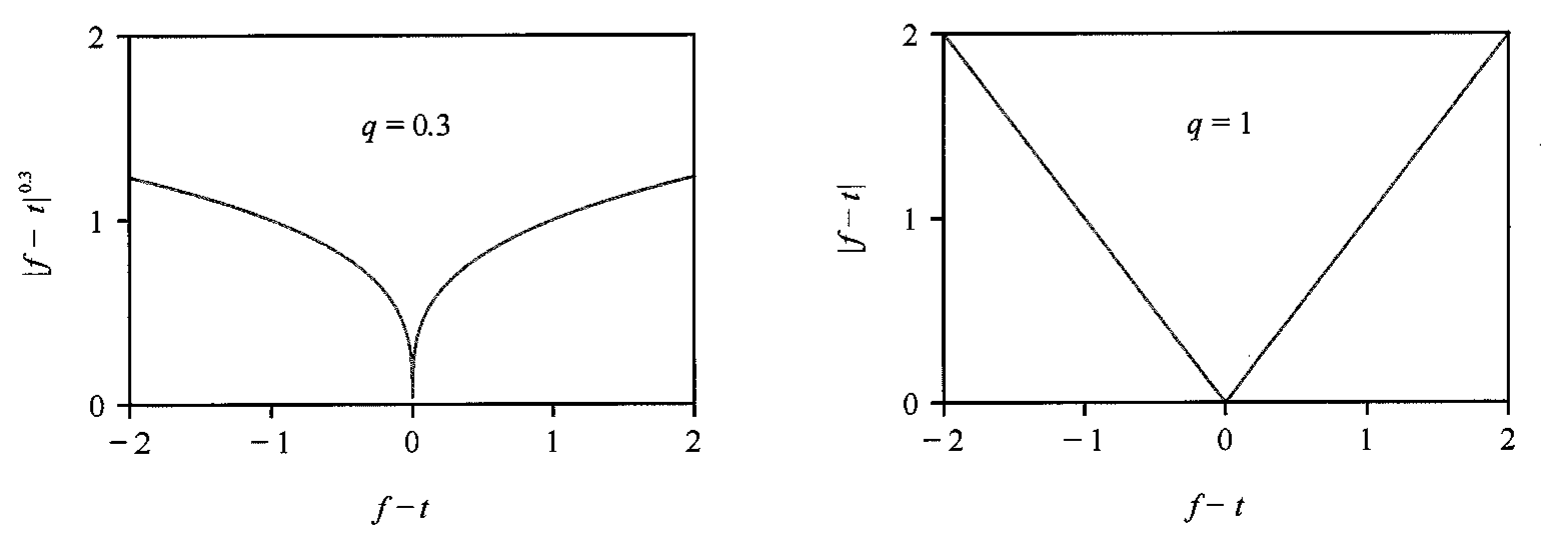
\includegraphics[width=0.92\textwidth]{ch04-fig4-6-loss-q-1.png}

  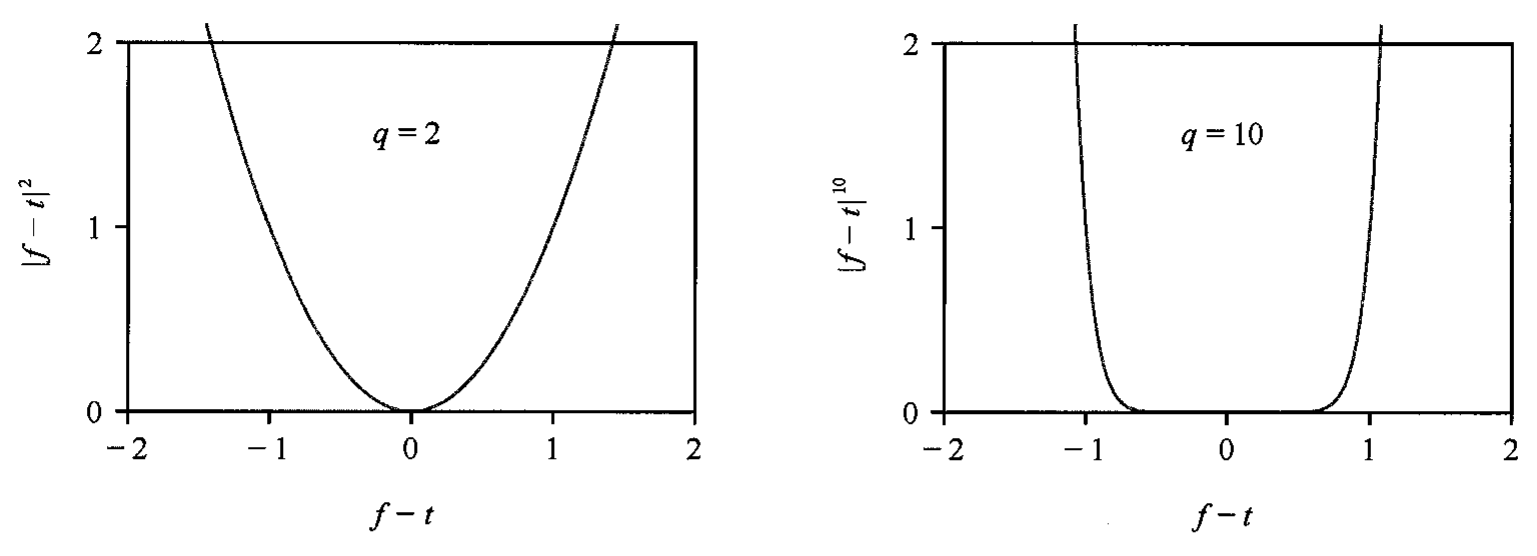
\includegraphics[width=0.92\textwidth]{ch04-fig4-6-loss-q-2.png}
  \caption{当$q$取不同值时，曲线$L_q=|f-t|^q$的示意图}
  \label{figure:ch04-损失曲线}
\end{figure}

Gauss噪声假设意味着给定$\boldsymbol{x}$时$t$的条件分布是单峰的，这对于某些应用来说可能是不合适的。在这种情况下，平方损失可能会导致结果变差，我们需要开发更复杂的其他方法。例如，我们可以通过使用混合Gauss分布来扩展这个模型，使其成为多峰条件分布（参见\cref{section:ch06-混合密度网络}）。这种情况在求解逆问题时会经常出现。本节重点讨论的是回归问题的决策理论，在下一章中，我们将在分类任务中引入类似的概念（参见\cref{section:ch05-决策理论}）。

\end{document}
